\section{IoT and Cloud Introduction}
The Internet of Things (IoT) involves the internet-connected devices we use to perform the processes and services that support our way of life. Another component set to help IoT succeed is cloud computing, which acts as a sort of front end. Cloud computing is an increasingly popular service that offers several advantages to IoT, and is based on the concept of allowing users to perform normal computing tasks using services delivered entirely over the internet.\\

Iot in cloud offers public cloud services can easily help the IoT area, by providing third party access to the infrastructure. Hence, the integration can help IoT data or computational components operating over IoT devices.\\

IoT devices need a lot of storage to share information for valuable purposes. Iot in cloud, like the StoneFly Cloud Connect to Microsoft Azure or we will use ThinkSpeak a free cloud service for IoT for student projects can provide customers with greater space which can increase as per the users demand. Helping to resolve the storage needs of customers.\\

The large amounts of data produced by IoT devices need extreme performance to interact and connect with one another. Iot in cloud provides the connectivity which is necessary to share information between the devices and make meaning from it at a fast pace.\\

Internet Cloud Computing infrastructures help IoT to give meaning to the greater amount of data generated. Users have no worry of buying greater or less storage. They can easily scale the storage as the data generated increases and pay for the amount of storage they consume with Internet Cloud Computing.




\section{IoT in Project}
he aim of this work is design and implements a distributed system for aquaculture water quality care through remote monitoring of dissolved oxygen, pH and temperature. This work will contribute remote monitoring distributed system through what is known as the Internet of Things to monitoring water quality in ponds. The system is modular, portable, low cost, versatile and allows sharing information through the cloud that can be used for the development and improvement of aquaculture activities. \\

The system can be implemented in aquaculture farms to be able to monitor in real time the most important physical-chemical variables of the water. With this having a faster response with respect to what actions to take when conditions arise in the water quality of the ponds\\

A monitoring system for water quality in aquaculture ponds is mentioned in the publication A Mobile Platform for Remote Monitoring of Water Quality. Mobile sensor platform for monitoring ponds. This system consists of the following architecture. It has the sensing node of each pond connected to a sink; this sink sends the information to a mobile application to have a visualization of the data in real time. This information is transmitted via GSM / 3G to the Internet, it can be monitored remotely and the information is stored in a database. In the results the data of the ponds were shown remotely and the measures were corroborated by the transport staff.\\


\section{Work Flow or Connectivity}

Here is the diagram which will help us to understand our work flow. Here is the images of all the sensors we will use.\\

pH Sensor : -\\

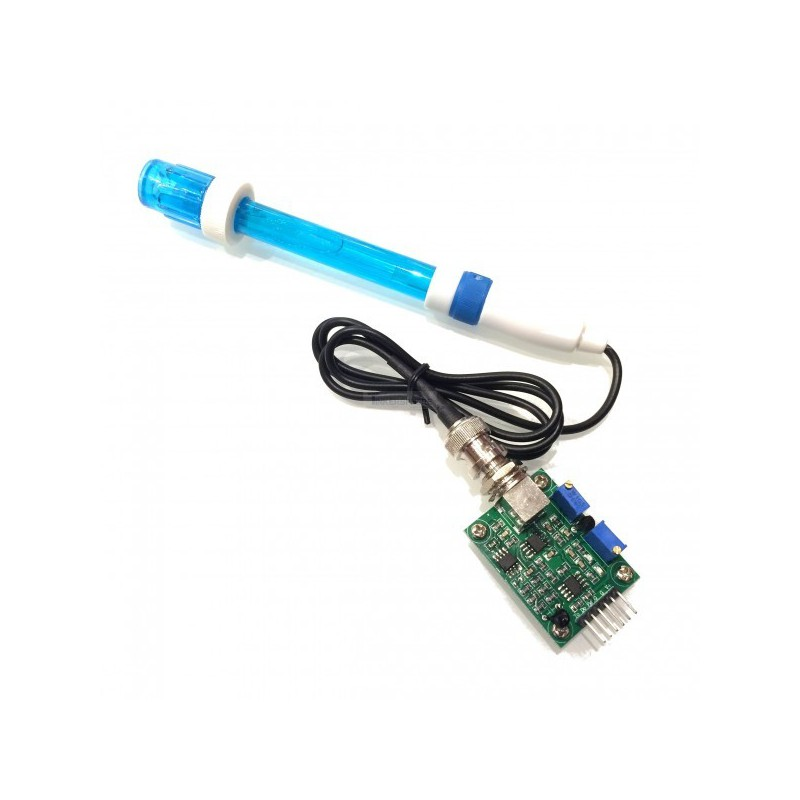
\includegraphics[width=0.6\textwidth]{images/ph sensor.jpg}\\

Temperature Sensor : -\\

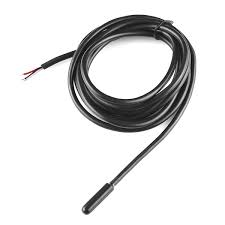
\includegraphics[width=0.6\textwidth]{images/temp sensor.jpeg}
\\

Work Flow Diagram :- \\

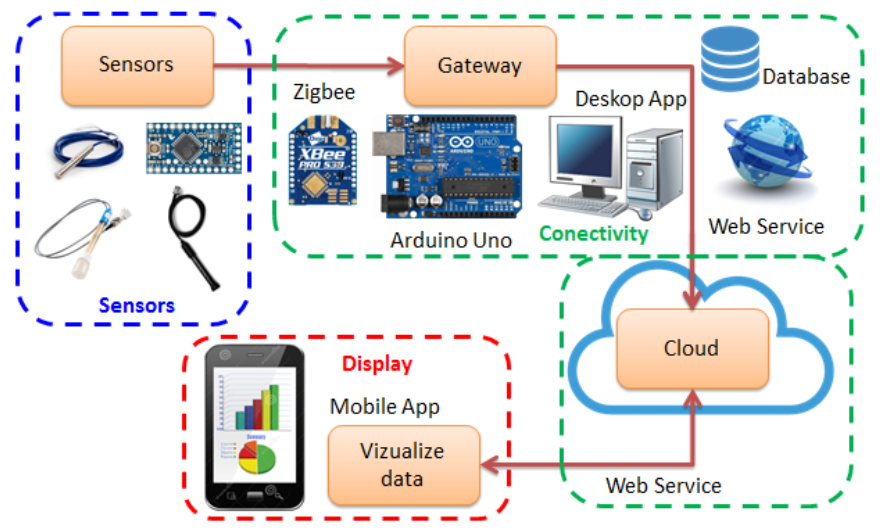
\includegraphics[width=0.6\textwidth]{images/workflow.png}\\



\subsection{Collect Data From Sensor}

In this section we will talk about first task of our workflow collect data from sensor and log it to console of arduino UNO. later we will send it to Cloud (ThinkSpeak for entire Project).\\

Below is the code of Collecting ph sensor and its connection and console it to COM Port console.\\

Figure : - 

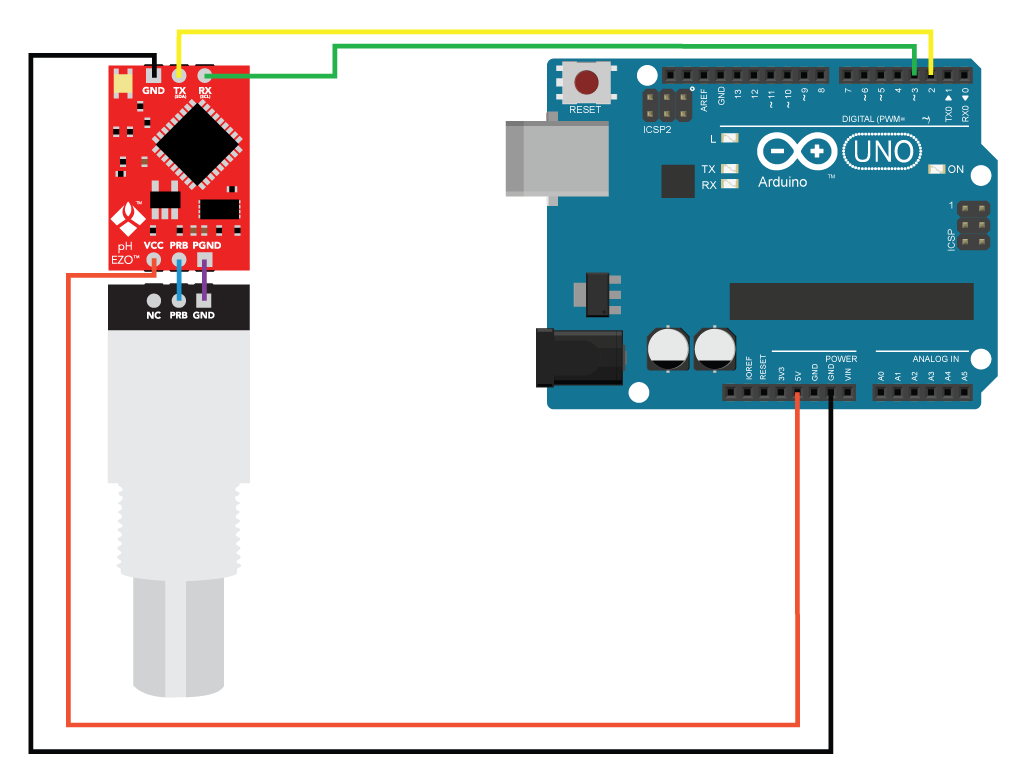
\includegraphics[width=0.6\textwidth]{images/ph-probe-calibration-wiring-diagram_YLRPvVdUwm.png}\\


\begin{lstlisting}[language=C++, caption={Arduino code for Ph sensor data}]
#include <Wire.h>
#include <LiquidCrystal_I2C.h>
LiquidCrystal_I2C lcd(0x27, 16, 2);
float calibration_value = 21.34;
int phval = 0; 
unsigned long int avgval; 
int buffer_arr[10],temp;
void setup() 
{
 Serial.begin(9600);
  lcd.init(); 
  lcd.begin(16, 2);
  lcd.backlight();
  lcd.setCursor(0, 0);
  lcd.print("   Welcome to      ");
  lcd.setCursor(0, 1);
  lcd.print(" Circuit Digest    ");
  delay(2000);
  lcd.clear();
}
void loop() {
 for(int i=0;i<10;i++) 
 { 
 buffer_arr[i]=analogRead(A0);
 delay(30);
 }
 for(int i=0;i<9;i++)
 {
 for(int j=i+1;j<10;j++)
 {
 if(buffer_arr[i]>buffer_arr[j])
 {
 temp=buffer_arr[i];
 buffer_arr[i]=buffer_arr[j];
 buffer_arr[j]=temp;
 }
 }
 }
 avgval=0;
 for(int i=2;i<8;i++)
 avgval+=buffer_arr[i];
 float volt=(float)avgval*5.0/1024/6;
 float ph_act = -5.70 * volt + calibration_value;
 lcd.setCursor(0, 0);
 lcd.print("pH Val:");
 lcd.setCursor(8, 0);
 lcd.print(ph_act);
 delay(1000);
}
\end{lstlisting}\\


Below is the code of Collecting temp. sensor and its connection and console it to COM Port console.\\

Figure : - 

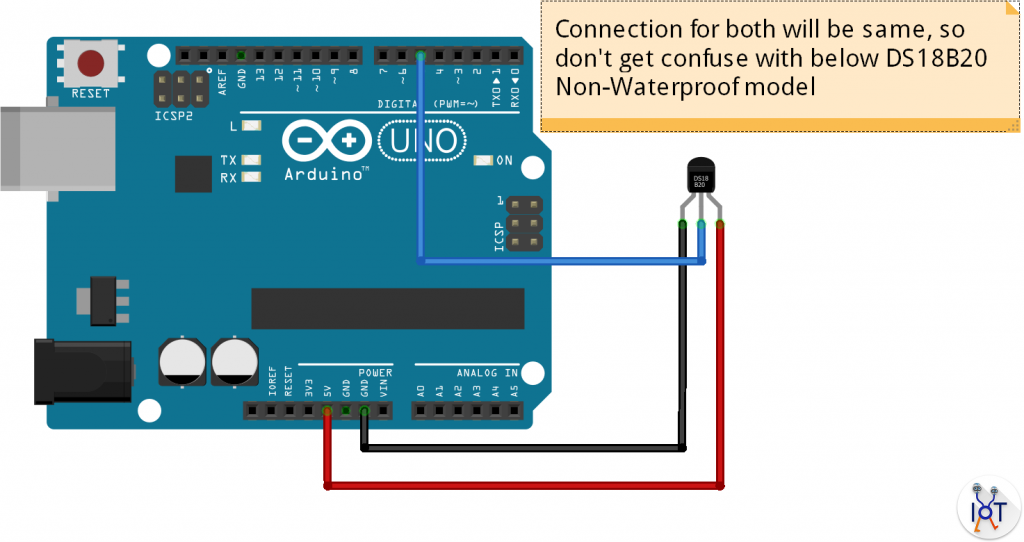
\includegraphics[width=0.6\textwidth]{images/temparature_sensor-www_iotboys_com_-1024x542_LqdcDeudhb.png}\\

\begin{lstlisting}[language=C++, caption={Arduino code for temp. sensor data}]
/********************************************************************/
// First we include the libraries
#include <OneWire.h> 
#include <DallasTemperature.h>
/********************************************************************/
// Data wire is plugged into pin 2 on the Arduino 
#define ONE_WIRE_BUS 2 
/********************************************************************/
// Setup a oneWire instance to communicate with any OneWire devices  
// (not just Maxim/Dallas temperature ICs) 
OneWire oneWire(ONE_WIRE_BUS); 
/********************************************************************/
// Pass our oneWire reference to Dallas Temperature. 
DallasTemperature sensors(&oneWire);
/********************************************************************/ 
void setup(void) 
{ 
 // start serial port 
 Serial.begin(9600); 
 Serial.println("Dallas Temperature IC Control Library Demo"); 
 // Start up the library 
 sensors.begin(); 
} 
void loop(void) 
{ 
 // call sensors.requestTemperatures() to issue a global temperature 
 // request to all devices on the bus 
/********************************************************************/
 Serial.print(" Requesting temperatures..."); 
 sensors.requestTemperatures(); // Send the command to get temperature readings 
 Serial.println("DONE"); 
/********************************************************************/
 Serial.print("Temperature is: "); 
 Serial.print(sensors.getTempCByIndex(0)); // Why "byIndex"?  
   // You can have more than one DS18B20 on the same bus.  
   // 0 refers to the first IC on the wire 
   delay(1000); 
} 
\end{lstlisting}\\

\subsection{Send data to cloud (ThingsSpeak)}

In this section we will make use of the data which we collected using both the sensor temp and ph and upload that data into the ThingsSpeak cloud which is cloud service offer by Matlab and it is free for student if you use it in limited conditions like minimum request to send data.\\

And from above section we know that the data from arduino is very fast reading like we get in every millisecond but we will upload data in 1 minute interval in cloud. to make minimum free usage for cloud.\\

Now Next thing which we will need to do to upload data in cloud is that we will need one wifi module which will connect to near by wifi hotspot and connect to cloud api to send data to channels in cloud. Below is the image of esp module device and code which make a connection of arduino and cloud\\

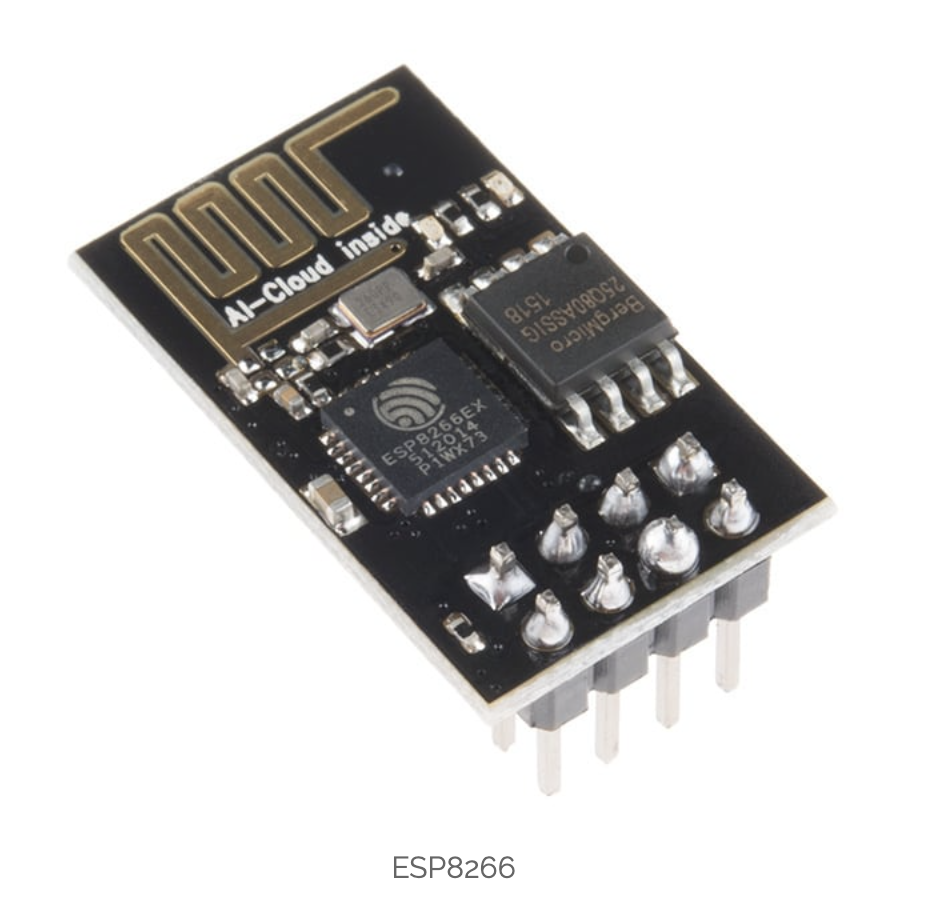
\includegraphics[width=0.6\textwidth]{images/esp.png}\\

\begin{lstlisting}[language=C++, caption={Arduino code for sending data to cloud}]

#include "ThingSpeak.h"
#include <ESP8266WiFi.h>

//------- WI-FI details ----------//
char ssid[] = "xxxxxxxxx"; //SSID here
char pass[] = "yyyyyyyyy"; // Passowrd here
//--------------------------------//

//----------- Channel details ----------------//
unsigned long Channel_ID = 12345; // Your Channel ID
const char * myWriteAPIKey = "ABCDEF12345"; //Your write API key
//-------------------------------------------//

const int Field_Number_1 = 1;
const int Field_Number_2 = 2;
String value = "";
int value_1 = 0, value_2 = 0;
int x, y;
WiFiClient  client;

void setup()
{
  Serial.begin(115200);
  WiFi.mode(WIFI_STA);
  ThingSpeak.begin(client);
  internet();
}

void loop()
{
  internet();
  if (Serial.available() > 0)
  {
    delay(100);
    while (Serial.available() > 0)
    {
      value = Serial.readString();
      if (value[0] == '*')
      {
        if (value[5] == '#')
        {
          value_1 = ((value[1] - 0x30) * 10 + (value[2] - 0x30));
          value_2 = ((value[3] - 0x30) * 10 + (value[4] - 0x30));
        }
      }
    }
  }
  upload();
}

void internet()
{
  if (WiFi.status() != WL_CONNECTED)
  {
    while (WiFi.status() != WL_CONNECTED)
    {
      WiFi.begin(ssid, pass);
      delay(5000);
    }
  }
}

void upload()
{
  ThingSpeak.writeField(Channel_ID, Field_Number_1, value_1, myWriteAPIKey);
  delay(15000);
  ThingSpeak.writeField(Channel_ID, Field_Number_2, value_2, myWriteAPIKey);
  delay(15000);
  value = "";

}

\end{lstlisting}\\

\subsection{Conclusion}

Now all data that we will need to make real time prediction is uploaded in cloud now we have to fetch data from this cloud and implement in mobile app and web app but before that we have to train our tensorflow model to make good model which can give us best predictions from our data. So, in the next section we will use Tensorflow Numpy Pandas and scikit to make prediction.